\documentclass[a4paper, 12pt]{article}%тип документа

%%%Библиотеки
	%\usepackage[warn]{mathtext}	
	\usepackage[T2A]{fontenc} % кодировка
	\usepackage[utf8]{inputenc} % кодировка исходного текста
	\usepackage[english,russian]{babel} % локализация и переносы
	\usepackage{caption}
	\usepackage{listings}
	\usepackage{amsmath,amsfonts,amssymb,amsthm,mathtools}
	\usepackage{wasysym}
	\usepackage{graphicx}%Вставка картинок правильная
	\usepackage{float}%"Плавающие" картинки
	\usepackage{wrapfig}%Обтекание фигур (таблиц, картинок и прочего)
	\usepackage{fancyhdr} %загрузим пакет
	\usepackage{lscape}
	\usepackage{xcolor}
	\usepackage[normalem]{ulem}
	\usepackage{hyperref}

%%%Конец библиотек




%%%Настройка ссылок
	\hypersetup
	{
		colorlinks=true,
		linkcolor=blue,
		filecolor=magenta,
		urlcolor=blue
	}
%%%Конец настройки ссылок


%%%Настройка колонтитулы
	\pagestyle{fancy}
	\fancyhead{}
	\fancyhead[L]{Лабораторная работа}
	\fancyhead[R]{Талашкевич Даниил, группа Б01-009}
	\fancyfoot[C]{\thepage}
%%%конец настройки колонтитулы



							\begin{document}
						%%%%Начало документа%%%%


%%%Начало титульника
\begin{titlepage}

	\newpage
	\begin{center}
		\normalsize Московский физико-технический институт \\(госудраственный 			университет)
	\end{center}

	\vspace{6em}

	\begin{center}
		\Large Лабораторная работа по электричеству\\
	\end{center}

	\vspace{1em}

	\begin{center}
		\large \textbf{Резонанс напряжений в последовательном контуре [3.2.2]}
	\end{center}

	\vspace{2em}

	\begin{center}
		\large Талашкевич Даниил Александрович\\
		Группа Б01-009
	\end{center}

	\vspace{\fill}

	\begin{center}
	Долгопрудный \\2021
	\end{center}
	
\end{titlepage}
%%%Конец Титульника



%%%Настройка оглавления и нумерации страниц
	\thispagestyle{empty}
	\newpage
	\tableofcontents
	\newpage
	\setcounter{page}{1}
%%%Настройка оглавления и нумерации страниц


					%%%%%%Начало работы с текстом%%%%%%
		
\section{Аннотация}
\textbf{Цель работы:} исследование резонанса напряжений в последовательном
колебательном контуре с изменяемой ёмкостью, получение амплитудно­
частотных и фазово-частотных характеристик, определение основных па­
раметров контура.\\
\textbf{В работе используются:} генератор сигналов, источник напряжения,
нагрузкой которого является последовательный колебательный контур с
переменной ёмкостью, двухканальный осциллограф, цифровые вольтмет­
ры.



\subsection{Теоретическое вступление и модель}

XXX

\subsection{Экспериментальная установка}

В данной работе изучаются резонансные явления в последовательном колебательном контуре (резонанс напряжений). Схема экспериментального стенда показана на рис. $1 .$ Синусоидальный сигнал от генератора поступает на вход управляемого напряжсением источника напрялсения (см., например, [3]), собранного на операционном усилителе, питание которого осуществляется встроенным блоком-выпрямителем от сети $\sim 220 \mathrm{~B}$ (цепь питания на схеме не показана). Источник напряжсения (источник с нулевым внутренним сопротивлением) обеспечивает с высокой точностью постоянство амплитуды сигнала $\mathcal{E}=\mathcal{E}_{0} \cos \left(\omega t+\varphi_{0}\right)$ на меняющейся по величине нагрузке - последовательном колебательном контуре, изображённом на рис. 1 в виде эквивалентной схемы.

Источник напряжения, колебательный контур и блок питания заключены в отдельный корпус, отмеченный на рисунке штриховой линией. На корпусе имеются коаксиальные разъёмы «Вход», «$U_1$» и «$U_{2}$», а также переключатель магазина ёмкостей $C_{n}$ с указателем номера $n=1,2, \ldots$ 7. Величины ёмкостей $C_{n}$ указаны на установке. Напряжение $\mathcal{E}$ на контуре через разъём «$U_1$» попадает одновременно на канал 1 осциллографа и вход 1-го цифрового вольтметра. Напряжение на конденсаторе $U_{C}$ подаётся через разъём «$U_2$» одновременно на канал 2 осциллографа и вход 2-го цифрового вольтметра.

\begin{center}

    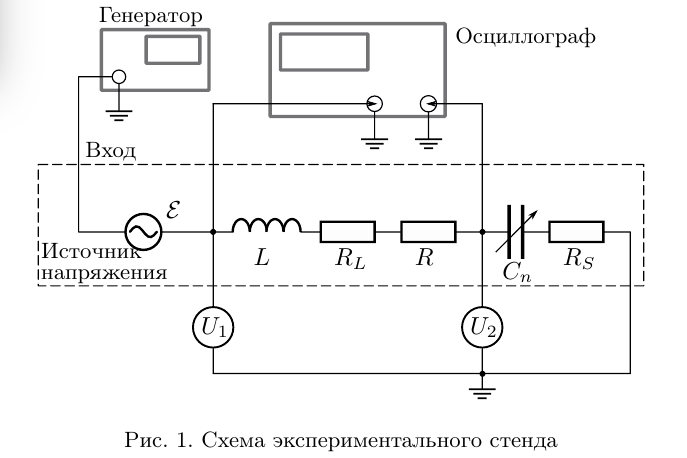
\includegraphics[scale=0.65]{pics/scheme1.png} \\
   % \textit{Рис. 1. Схема установки}

\end{center}

\section{Ход работы}
\begin{enumerate}
\item Подготавливаем установку к работе и включаем приборы.
\item Выставляем на входе контура напряжение $E = 100~\text{мВ}$, в течении всей работы поддерживая его постоянным.
\item Добиваемся получения двух отцентрованных синусоид на осциллографе. Убеждаемся, что одна из синусоид при изменении частоты $f$ генератора меняет амплитуду относительно начала координа, в то время как амплитуда другой не меняется с погрешностью не более 1\%.
\item Для контуров с семью различными ёмкостями, меняя их с помощью переключателя на
блоке, измеряем резонансные частоты $f_{0n}$ и напряжения $U_C(f_{0n})$. Регистрируйем также
напряжения $E(f_{0n})$, игнорируя отклонения в пределах относительной погрешности 1%.
\item Для контуров ёмкостями $C_1 = 25~\text{нФ}$ и $C_1 = 57.2~\text{нФ}$ снимаем амплитудно-частотные характеристики $U_C(f)$ (16-17 точек
в сумме по обе стороны от резонанса) при том же напряжении $E$.

%%%%%%%%%%%%%5

\begin{table}[h]
\begin{tabular}{|c|c|c|c|c||c|c|c|c|c|}
\hline \multicolumn{5}{|c||}{$C_{1}=XX$ нФ} & \multicolumn{5}{c|}{$C_{4}=XX$ нФ } \\
\hline$n$ & $f$, кГц & $\sigma_{f}$, кГц & $A$, B & $\sigma_{A}$, B & $n$ & f, кГц & $\sigma_{f}$, кГц & A, B & $\sigma_{A}$, B \\
\hline 1   &  &  &  &  &  &  &  &  &  \\
\hline 2   &  &  &  &  &  &  &  &  &  \\
\hline 3   &  &  &  &  &  &  &  &  &  \\
\hline 4   &  &  &  &  &  &  &  &  &  \\
\hline 5   &  &  &  &  &  &  &  &  &  \\
\hline 6   &  &  &  &  &  &  &  &  &  \\
\hline 7   &  &  &  &  &  &  &  &  &  \\
\hline 8   &  &  &  &  &  &  &  &  &  \\
\hline 9   &  &  &  &  &  &  &  &  &  \\
\hline 10  &  &  &  &  &  &  &  &  &  \\
\hline 11  &  &  &  &  &  &  &  &  &  \\
\hline 12  &  &  &  &  &  &  &  &  &  \\
\hline 13  &  &  &  &  &  &  &  &  &  \\
\hline 14  &  &  &  &  &  &  &  &  &  \\

\hline
\end{tabular}
\caption{таблица X}
\end{table}

%%%%%%%%%%%%


\newpage
\item Для тех же двух контуров снимите фазово-частотные характеристики $\varphi_C(f)$ ($\sim 10-15$ точек в сумме по обе стороны от резонанса) при том же
напряжении $E$.

%%%%%%%%%%%

\begin{table}[h]
\begin{center}
\begin{tabular}{|c|c|c||c|c|c|}
\hline \multicolumn{3}{|c||}{$C_{1}=XX$ н $\Phi$} & \multicolumn{3}{c|}{$C_{4}=XX \mathrm{H} \Phi$} \\
\hline$n$ & $f$, кГ & $-\varphi / \pi$ & $n$ & $f$, кГц & $-\varphi / \pi$ \\
\hline 1  &   &    & 1  &   & \\
\hline 2  &   &    & 2  &   & \\
\hline 3  &   &    & 3  &   & \\
\hline 4  &   &    & 4  &   & \\
\hline 5  &   &    & 5  &   & \\
\hline 6  &   &    & 6  &   & \\
\hline 7  &   &    & 7  &   & \\
\hline 8  &   &    & 8  &   & \\
\hline 9  &   &    & 9  &   & \\
\hline 10 &   &    & 10 &   & \\
\hline
\end{tabular}
\end{center}
\caption{таблица X}
\end{table}

%%%%%%%%%%


\end{enumerate}
\newpage

\section{Обработка результатов}

\begin{itemize}

\item XXX

\item XXX

\item XXX

\item XXX

\item XXX

\end{itemize}

XXX

\section{Графики и таблицы}

XXX

\section{Вывод}

XXX

\section{Литература}

\begin{enumerate}
\item \textbf{Лабораторный практикум по общей физике:} Учебное пособие. В трех томах. Т. 2. Электричество и магнетизм /Гладун А.Д., Александров Д.А., Берулёва Н.С. и др.; Под ред. А.Д. Гладуна - М.: МФТИ, 2007. - 280 с.
\end{enumerate}		
		
					
\end{document}